Die Bibliothek Anwendung soll in eine andere Hauptanwendung integriert werden. 
Die Bibliothek soll sich genauso gegenüber der getesteten Ladesäule verhalten, wie eine Standalone-Anwendung. 
Somit soll die Datenbank-Schnittstelle simuliert werden. 
Es ist vorgegeben die Logs von der Bibliothek aufzuzeichnen, damit ist eine simulierte Filesystem-Schnittstelle notwendig.
Die Bibliothek wird direkt (mittels Methodenaufrufen) über UI-Controller angesteuert, 
somit wird die HTTP-Schnittstelle nicht verwendet. 

Die Anwendung lässt sich wie folgt darstellen (Die blaue Farbe stellt simulierte Komponenten
dar, die schwarze Farbe stellt fehlende Komponente dar):
\import{./images/solutions}{Library}

\newpage
Die Struktur der Bibliothek als Klassendiagramm sieht wie folgt aus:

\begin{figure}[H]
    \centering
    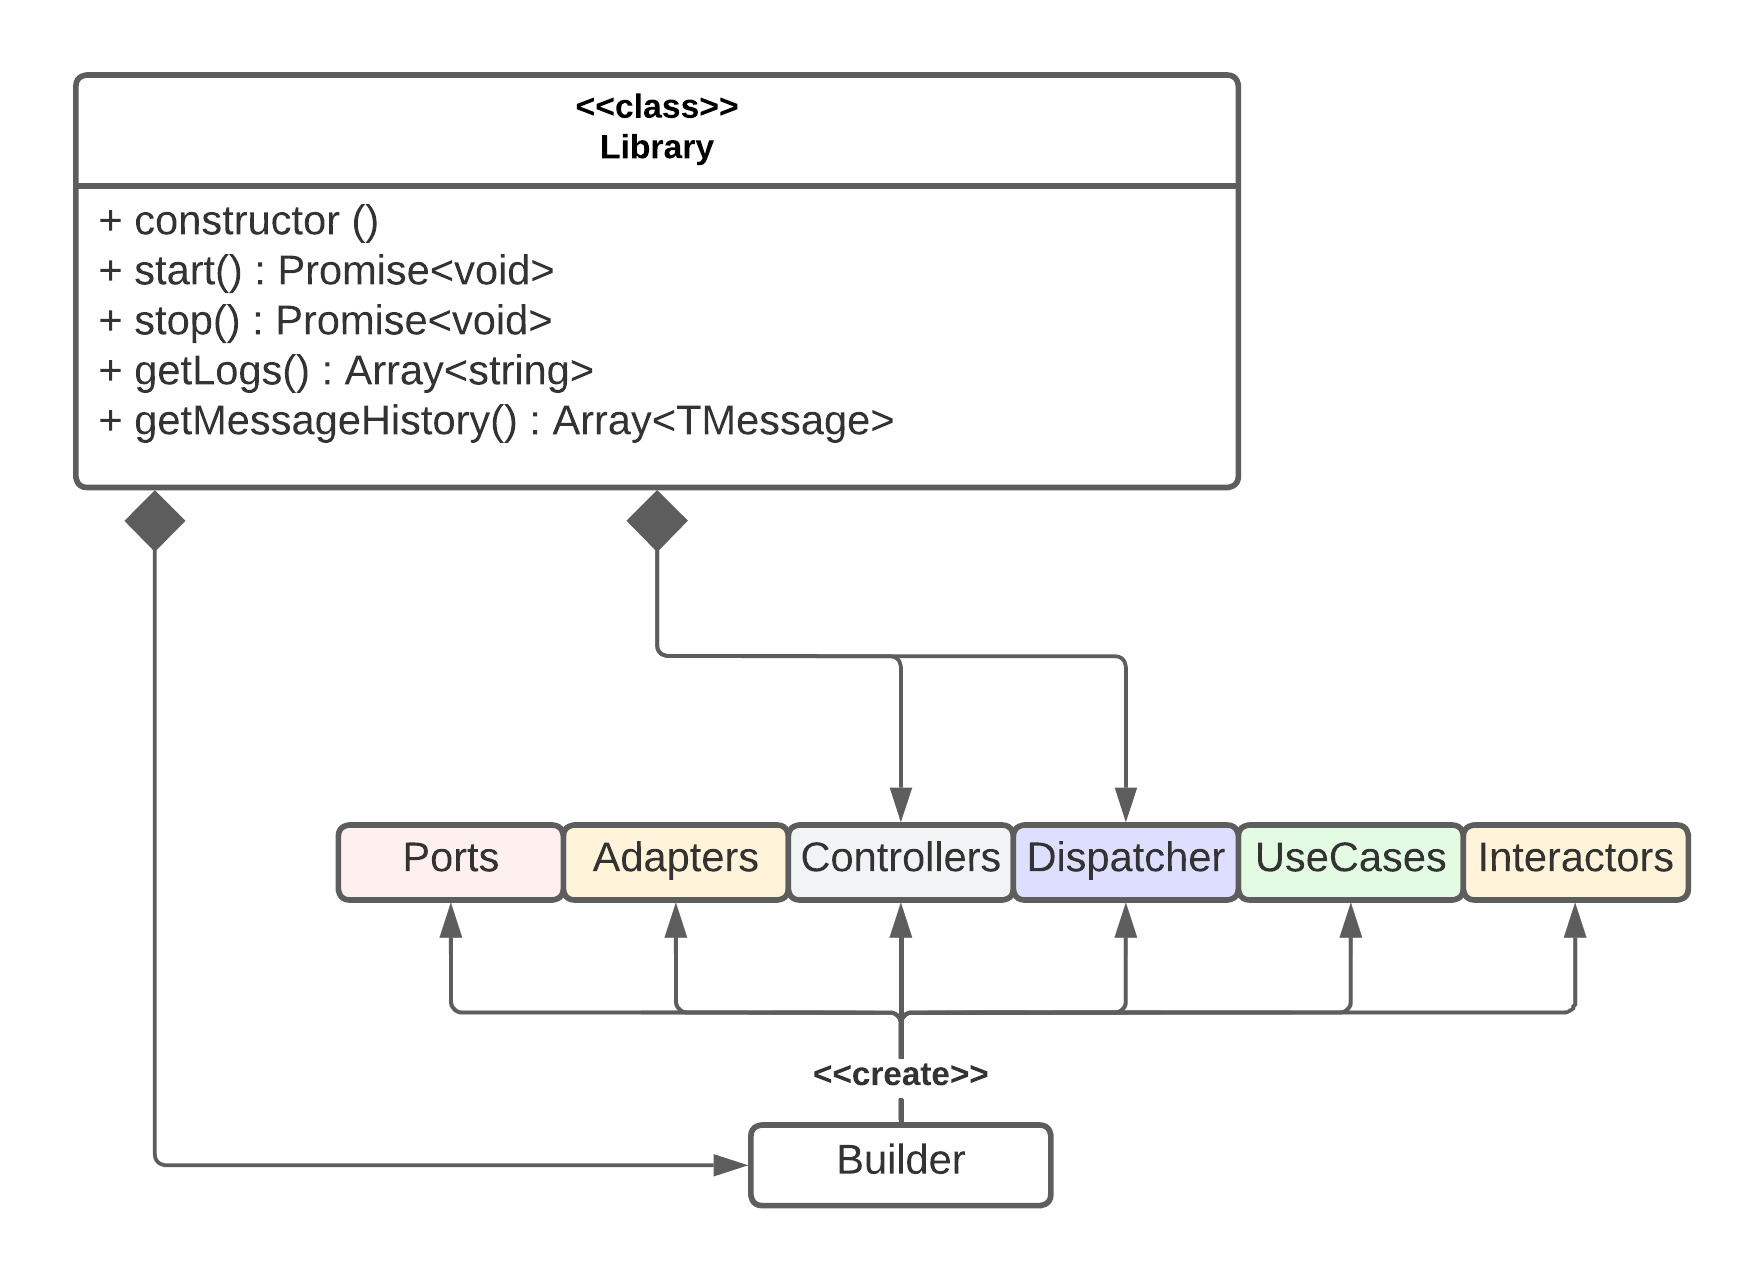
\includegraphics[width=0.8\textwidth]{./images/LibraryKlassenDiagramm.png}
    \caption[Struktur der Bibliothek]{Struktur der Bibliothek}
    \label{fig:LibraryClassDiagramm}
\end{figure}